\documentclass{article}

\usepackage{geometry}
\geometry{a4paper, scale=0.8}

\usepackage{graphicx}
\usepackage{float}

\usepackage{ctex}

\title{Progress Report 3: High Availability}
\author{Group "200"\\YiDai 2017013562\\ZhaohengLi 2017050025}

\begin{document}
\maketitle



\section{对于负载均衡相关内容的调研总结}
\subsection{算法性质}
按负载均衡采用的算法来区分,可以分为动态和静态两类,静态负载均衡按照实现给定的权重(概率)
分配任务,而动态负载均衡算法要考量实时负载,其中包括当前延迟或链接数量。
在我们常用的方法中,轮询法、加权轮询法、随机法就属于静态,而最小连接法就属于动态。
然而负载均衡真正的多样性来自于提供该服务的来源和对象不同:
\subsection{来源不同}
当我们从设备的角度考量,有硬件和软件两种解决方案。成熟的硬件负载均衡,如F5,可以对外部展现虚拟服务器地址,通过NAT将连接转到适合的真实服务器上。软件负载均衡则有Nginx等提供的服务,如Nginx在应用层通过upstream模块实现均衡。

硬件和软件实现各有优劣,硬件实现可以直接通过交换机实现,与系统无关,但其只能从网络层判断负载,存在一定限制;软件负载配置简单、自带日志实现,且实现成本较低,方便实现硬件资源的高效利用,但负载能力受服务器性能的影响。当然,无论硬件和软件,都有一系列的算法可以配置,且内部也存在分化(如软件负载均衡中的LVS和Nginx)
\subsection{对象不同}
负载均衡对象有不同体现在这里:我们是对链路实现负载均衡,还是对服务器、广域网。我们这里主要讨论的是服务器的负载均衡,但如链路负载均衡技术,包括就近链路选择、实时探测等算法,在一些服务中也会被使用。




\section{负载均衡实现}
我们接下来使用Nginx的负载均衡,所以主要描述其中的算法,其默认使用轮询,还有weight(加权轮询)、ip\_hash(按访问IP的哈希结果分配,方便建立稳固的联系,在购物类应用中颇有作用),fair(根据页面大小、加载时间长短来均衡),url\_hash(按访问url的哈希结果分配请求,提高后端缓存服务器的效率)。可见这些算法各有适用场景。
\subsection{我们的负载均衡方法}
我们采用fair策略,根据页面大小、加载时间长短智能的进行负载均衡。该方法在初始的nginx中并没有支持,需要我们手工添加附加包、修改原先的结构体来实现新算法。

我们原计划在原服务器中建立四个服务,提供四个端口,但为了接近真实的负载均衡,我们后续加入了一台腾讯云单核服务器,与原计划效果进行对比。



\subsection{负载均衡实现检验}
我们分别核验后端多个服务的访问日志、停止一部分服务来检验负载均衡的效果。
我们暂时中断175.24.30.4上的所有服务,此时我们的网页仍能正常使用,且因为剩下的服务提供数据更快,延迟更小了。而观察所有后端日志,可以发现

\subsection{负载测试}
我们使用JMETER的取样器、监听器,实现不同的请求,查看单位时间延迟和吞吐量。
我们测试20个线程,Rame-Up Period(启动时间,即所有线程全部启动花费时间(s))设为10秒。我们需要大概十分钟到十五分钟完成一次一般的负载测试、获得稳定的结果。

我们可以生成数字和图形形式的报表。
\begin{figure}[H]
\centering
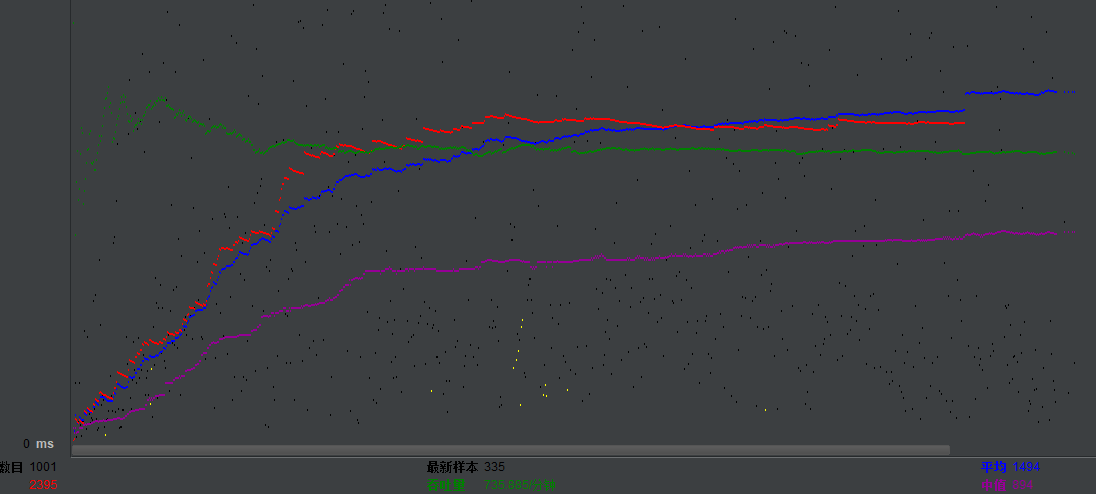
\includegraphics[width=0.85\textwidth]{progress-report-3/graph.png}
\end{figure}
\begin{figure}[H]
\centering
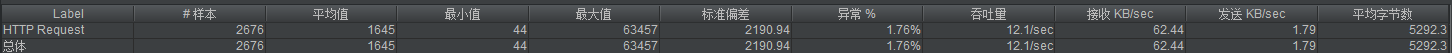
\includegraphics[width=0.85\textwidth]{progress-report-3/figure.png}
\end{figure}
\subsubsection{单场景测试}
我们暂时只加入全国信息查询,获得结果:平均延迟为1811ms,吞吐量为10.4/sec。
\subsubsection{多场景测试}
我们同时加入了新闻查询、谣言查询和全国疫情信息查询三个http请求配置元件。在单线程中,我们发现其latency具有显著差别,全国疫情信息延迟最高,是另两个的若干倍。多场景测试比较贴近实际情况,用户的具体请求有差别。

在我们Nginx使用朴素轮询策略时,我们得到的平均延迟为1655ms,吞吐量为11.9/sec,我们使用加载时间适应策略时,得到的平均延迟为1569ms,吞吐量为12.1/sec。

为何表现基本相近?原因在于当我们使用相同的服务器、不同的服务器有同样的工作环境,此时并不会产生不同服务之间延迟的明显差异,所以两种方法不会有太大差别。

当我们引入一台新的服务器呢?

我们有一台腾讯云服务器已结束其他用途的使用,现在加以利用。我们发现引入新的服务器反而使得整体速度变慢,通过ping、查看JMeter的报告,我们发现是该服务器上挂载服务的通信时间过长所致。在这种情况下,理想的方式是将其作为备用服务器。

不过这种情况下我们也有手段来测试fair策略和朴素轮询策略的优劣了。我们在朴素轮询策略下,获得的平均延迟为4075ms,吞吐量为4.2/sec;而fair策略下,我们获得的平均延迟为2930ms,吞吐量为5.3/sec。说明fair策略确实做到了考量页面和加载时间来分配负载。

\section{各个服务的访问日志}

下图是在服务器上分别开设于不同的端口的多个不同服务的访问日志。

\begin{figure}[H]
\centering
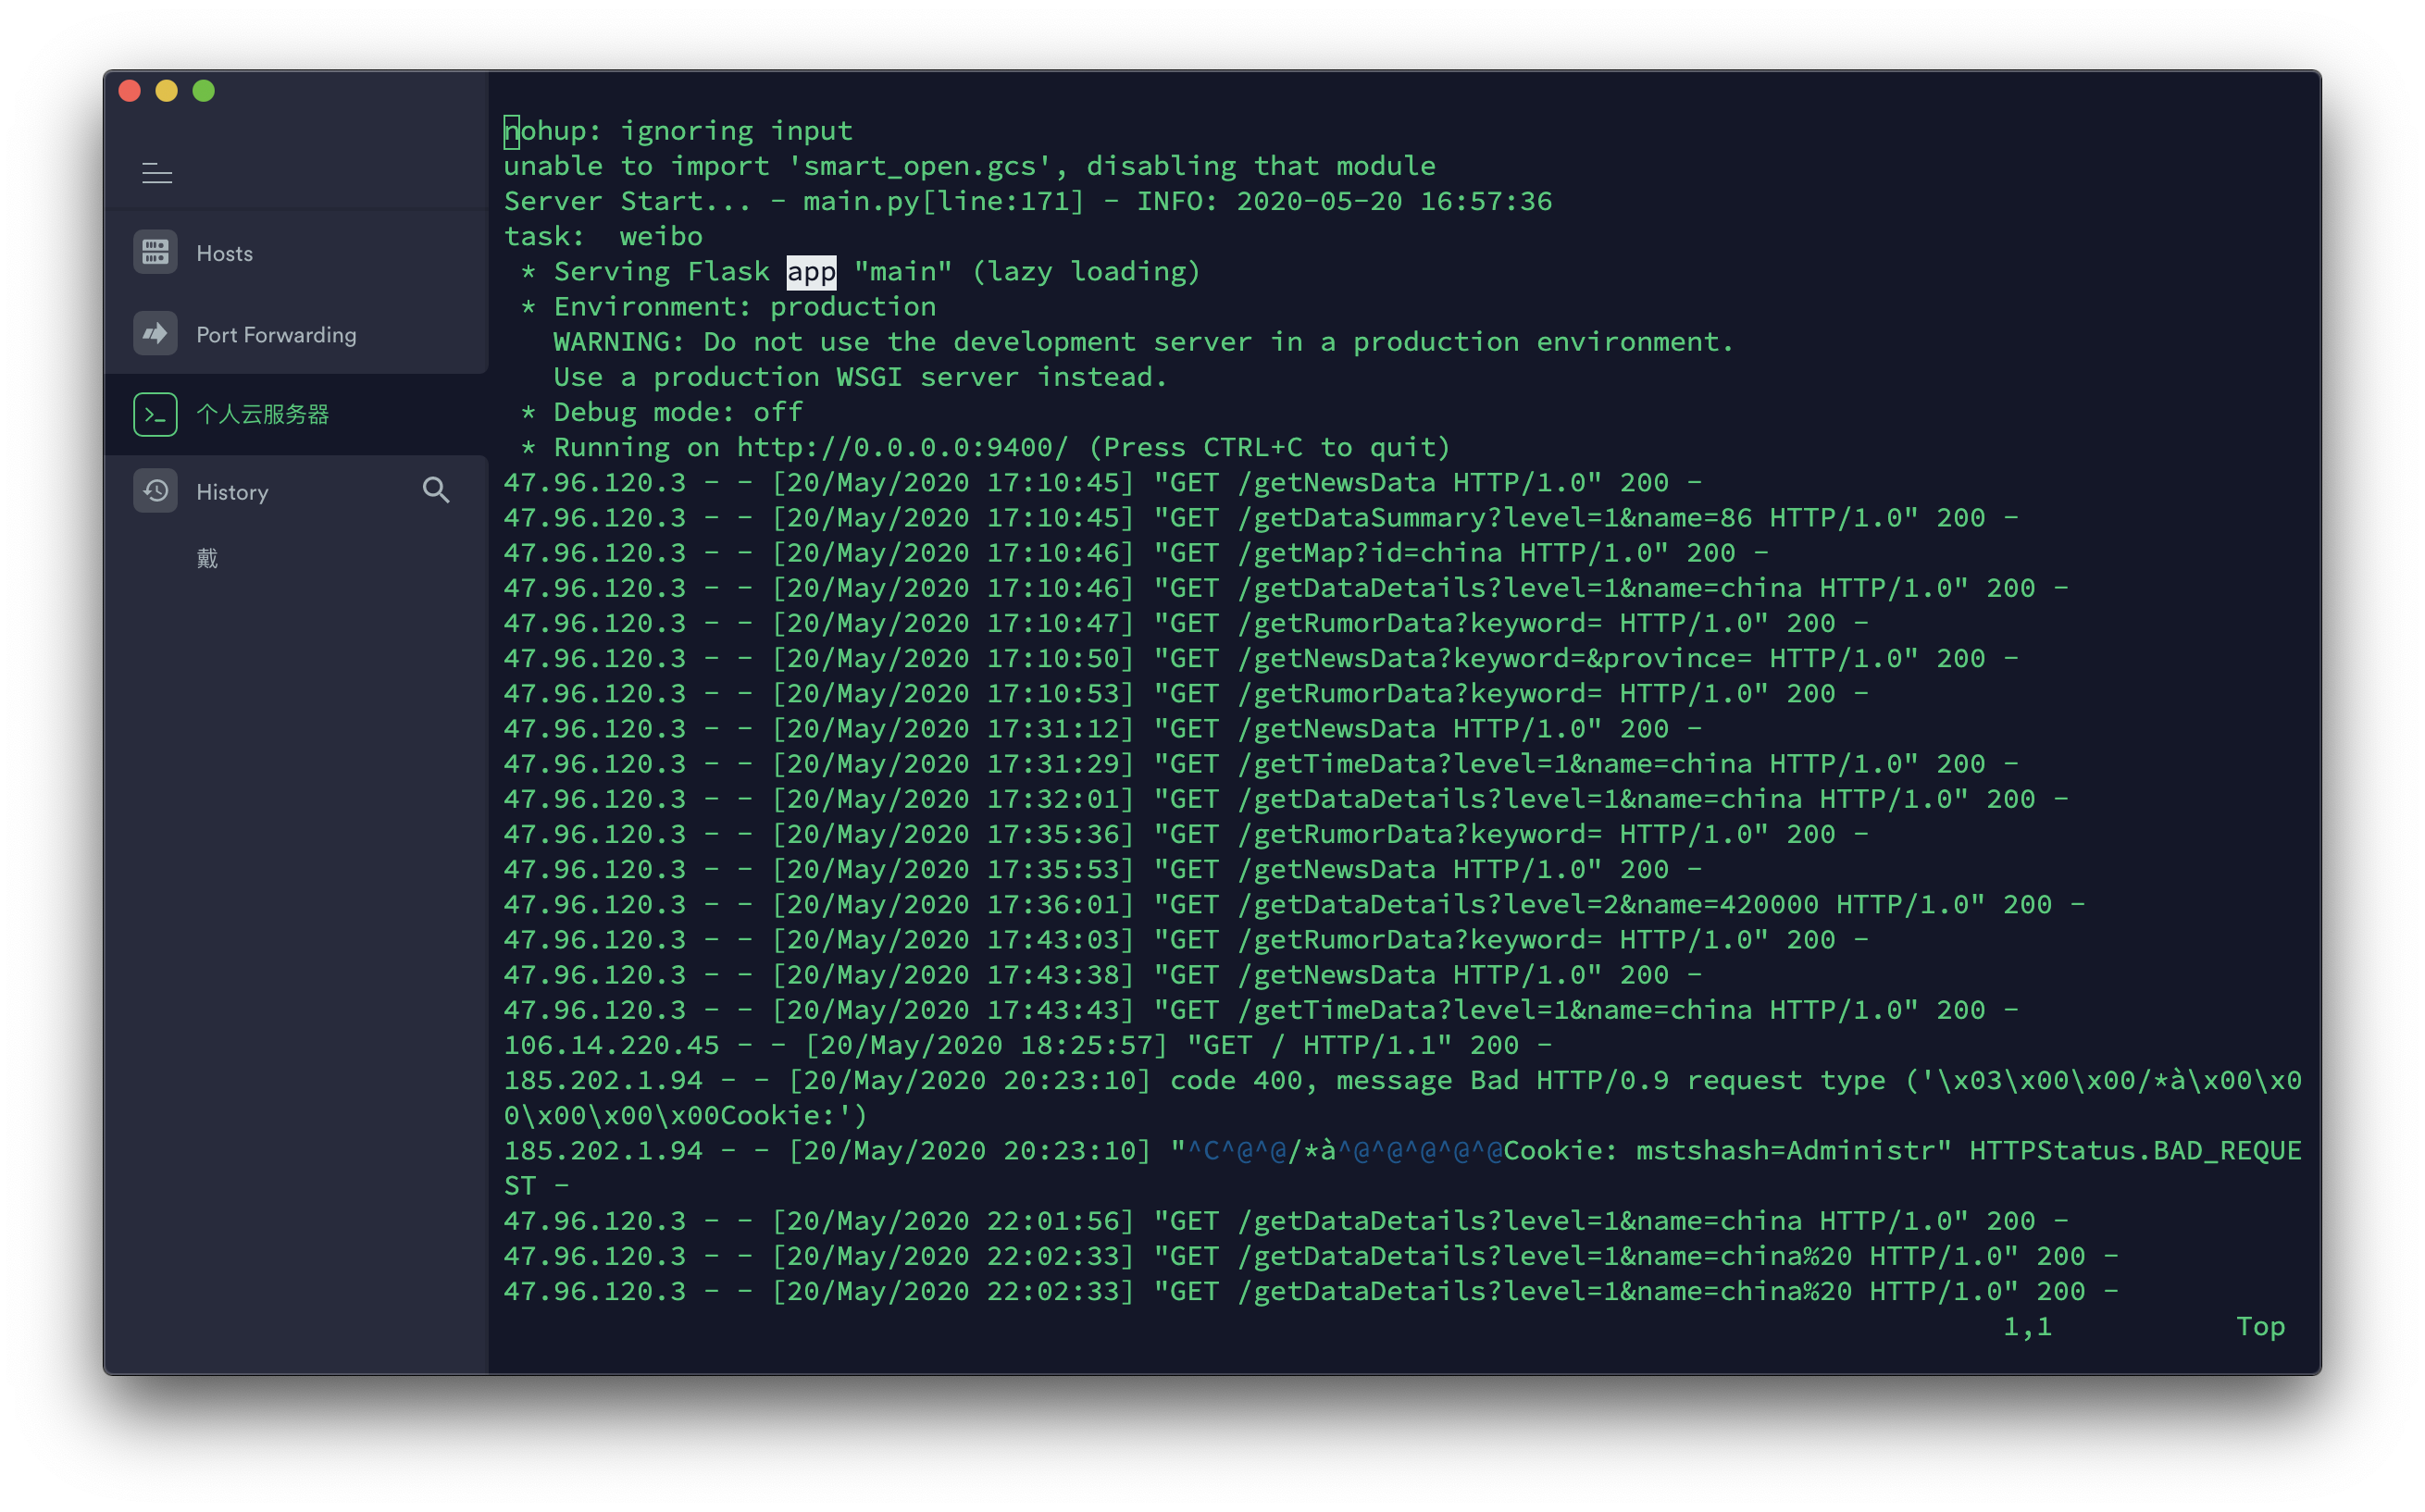
\includegraphics[width=0.6\textwidth]{progress-report-3/log0.png}
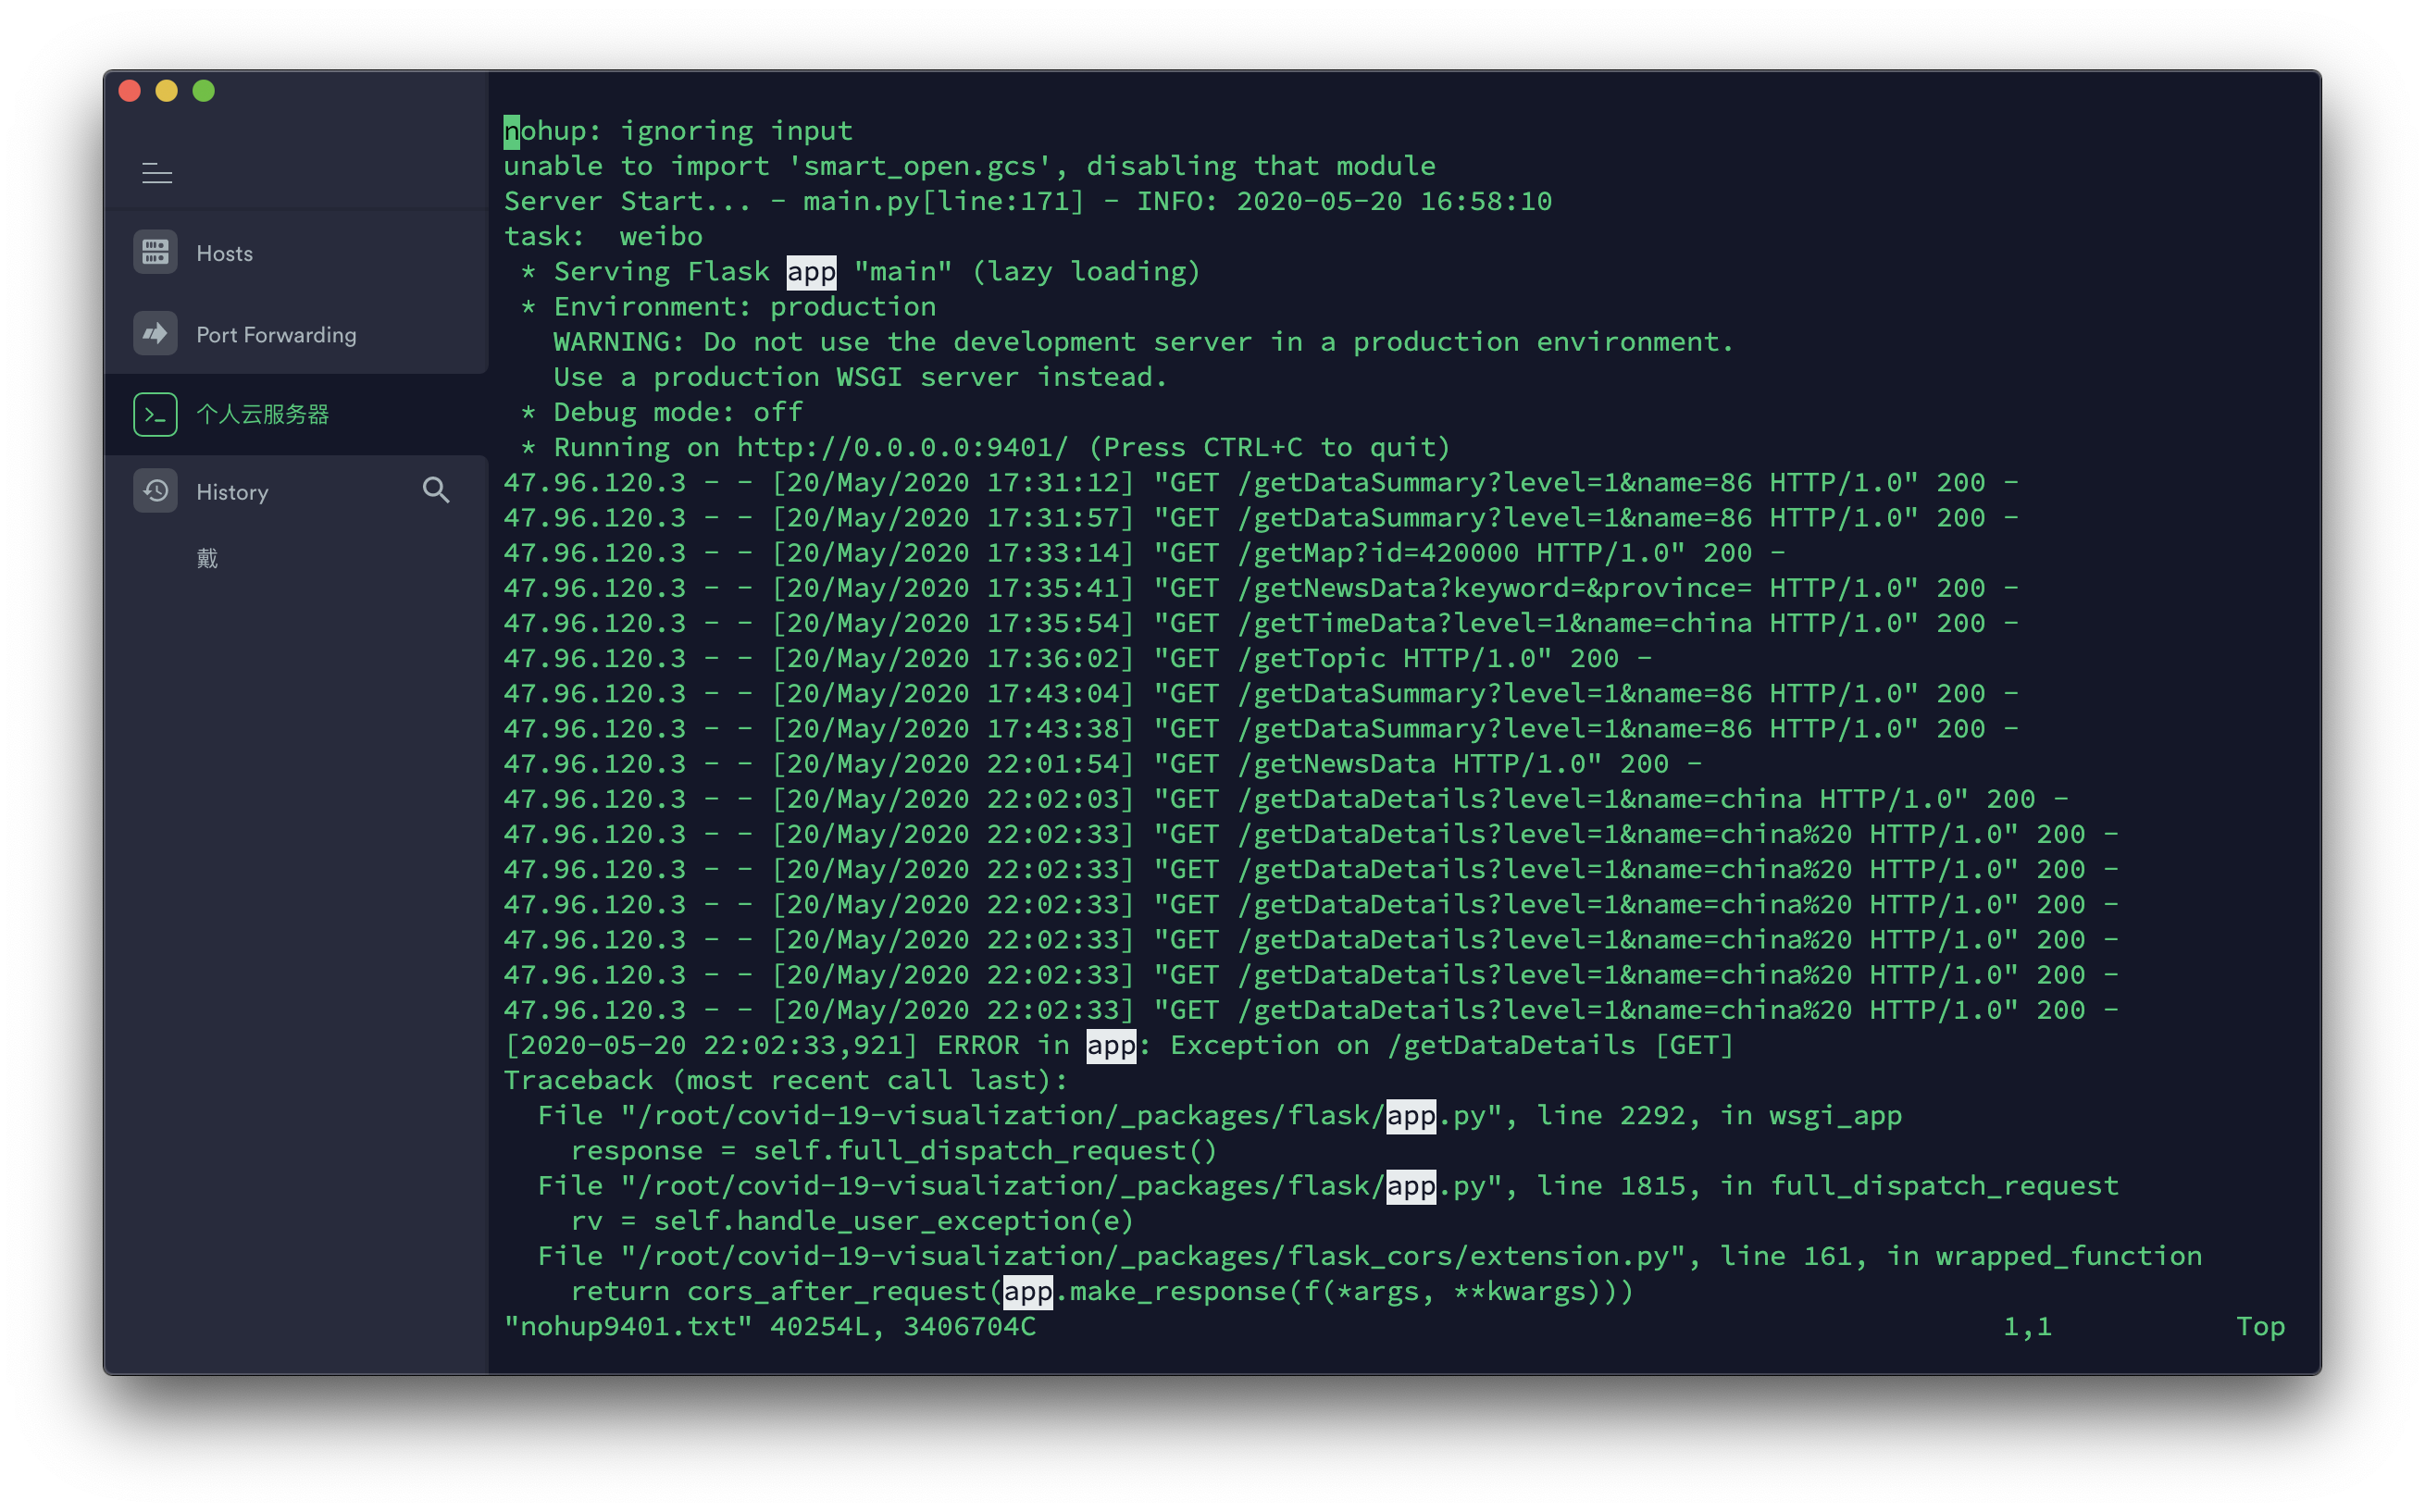
\includegraphics[width=0.6\textwidth]{progress-report-3/log1.png}
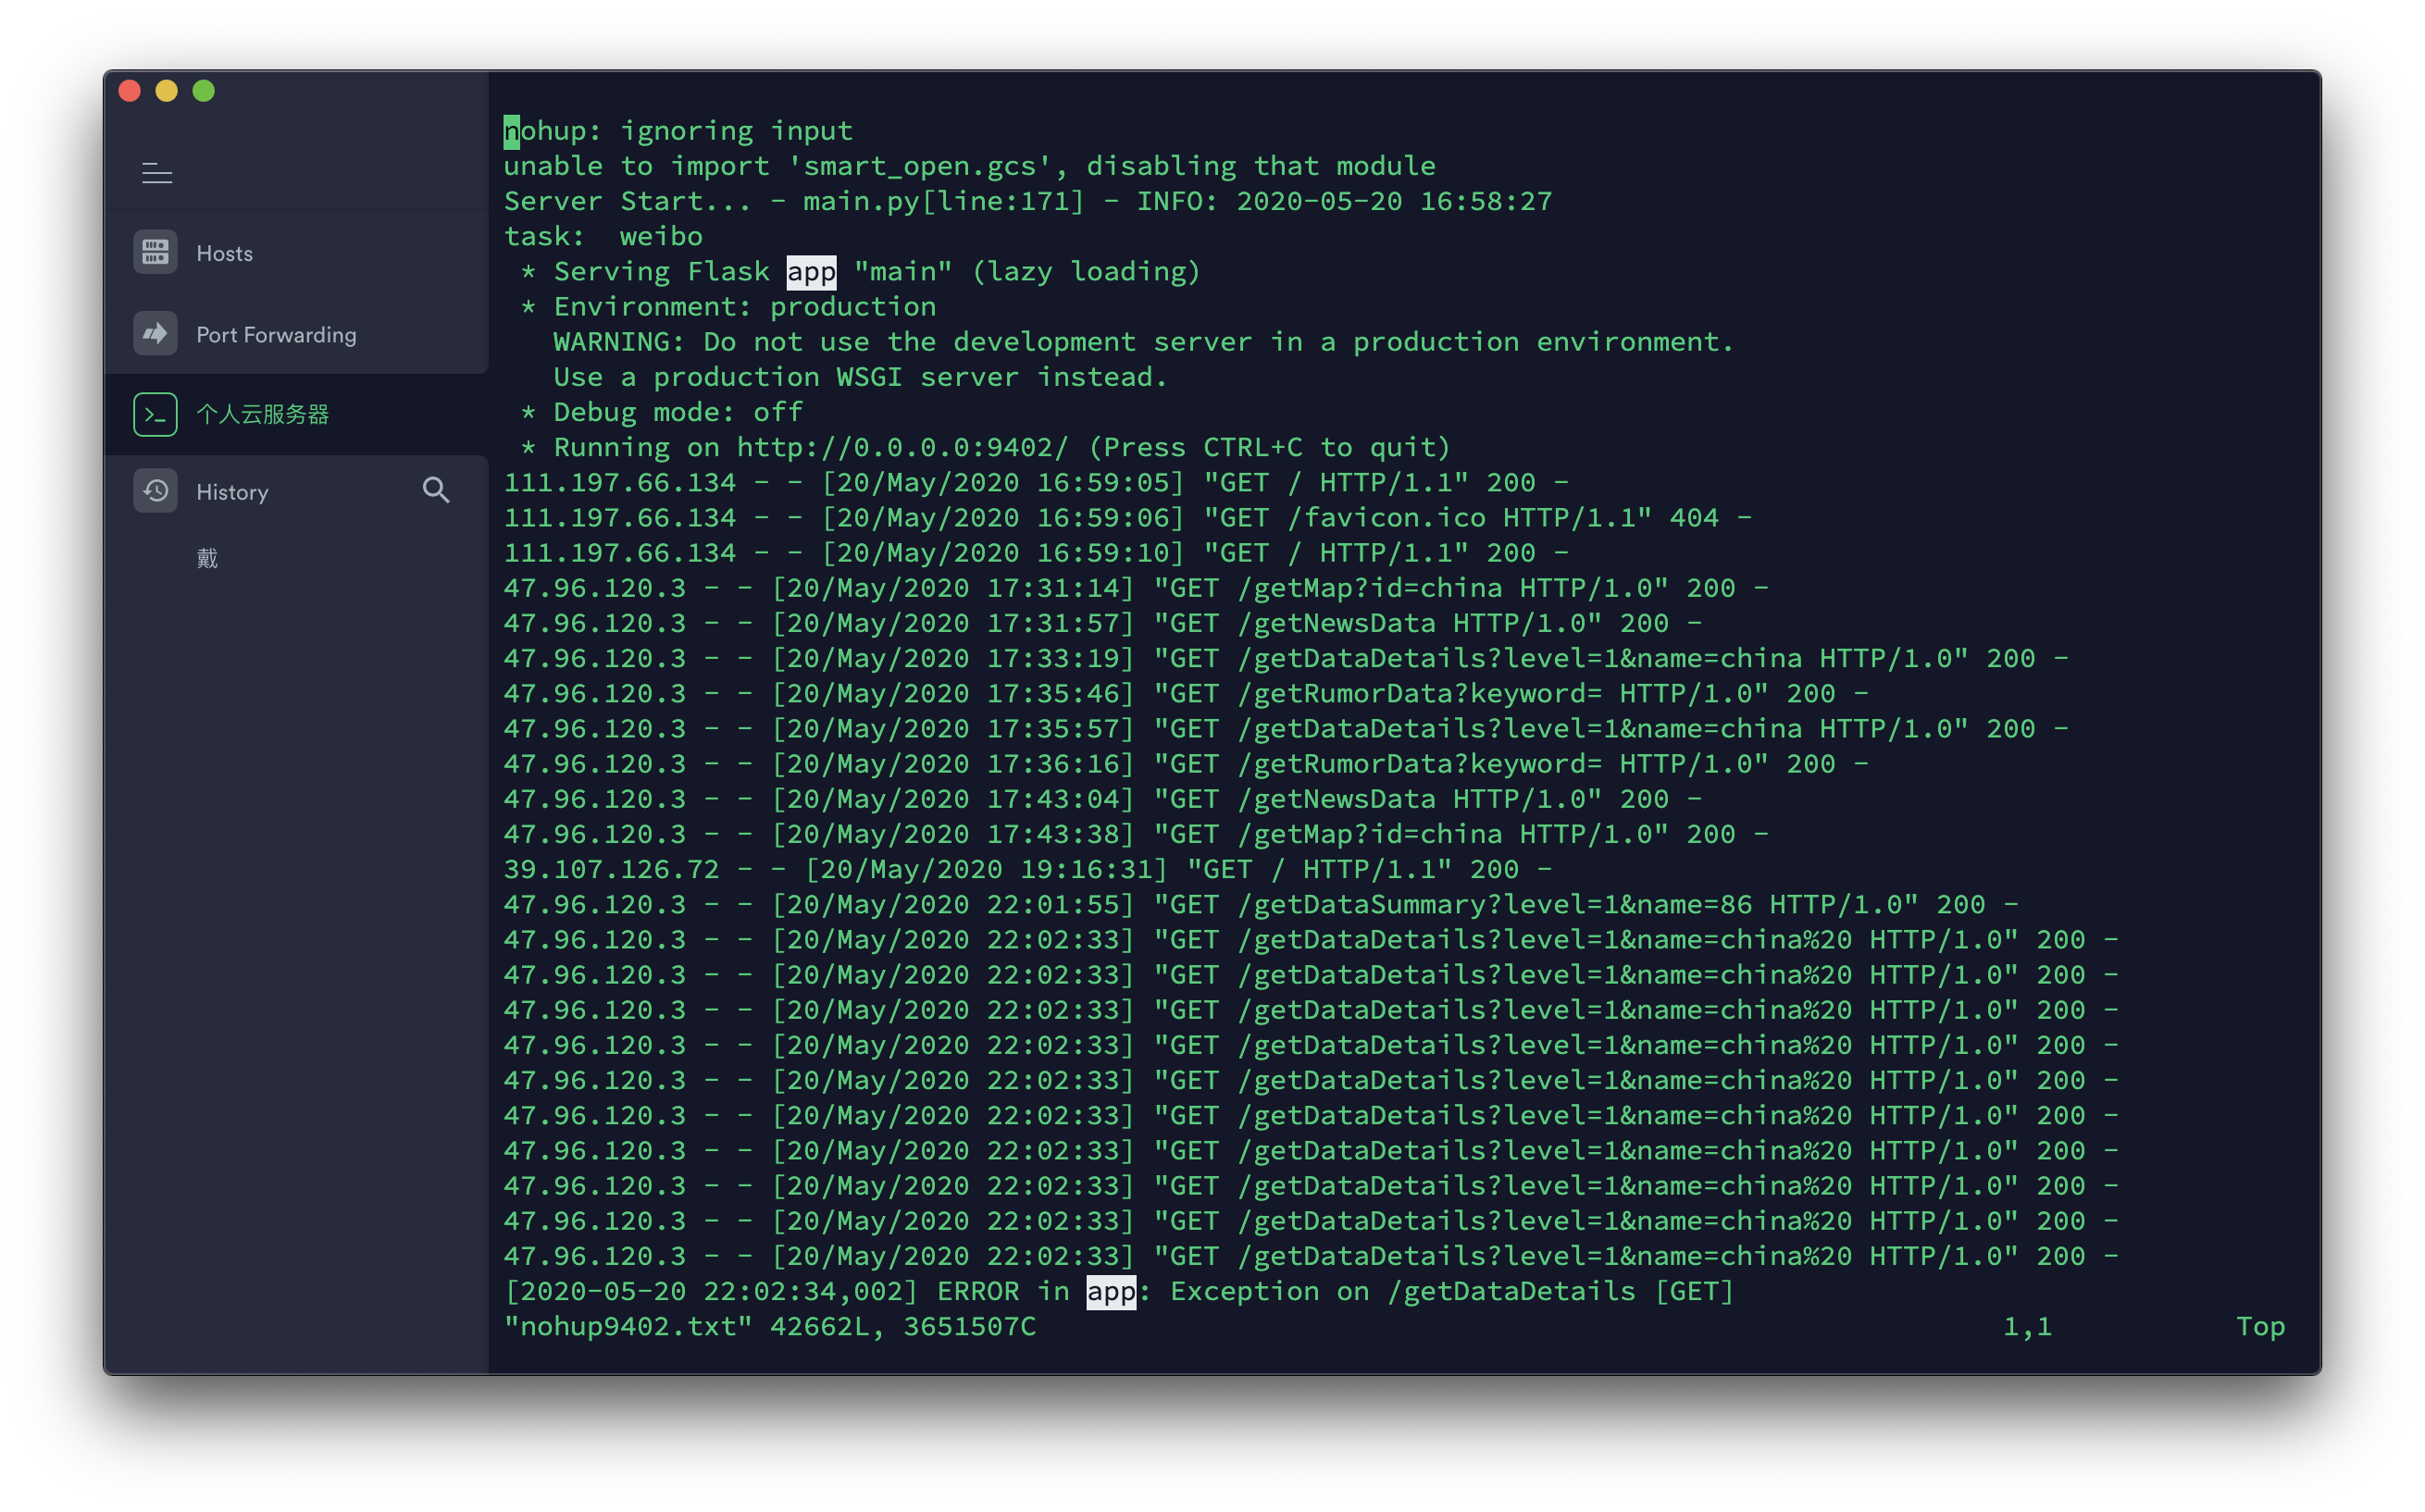
\includegraphics[width=0.6\textwidth]{progress-report-3/log2.png}
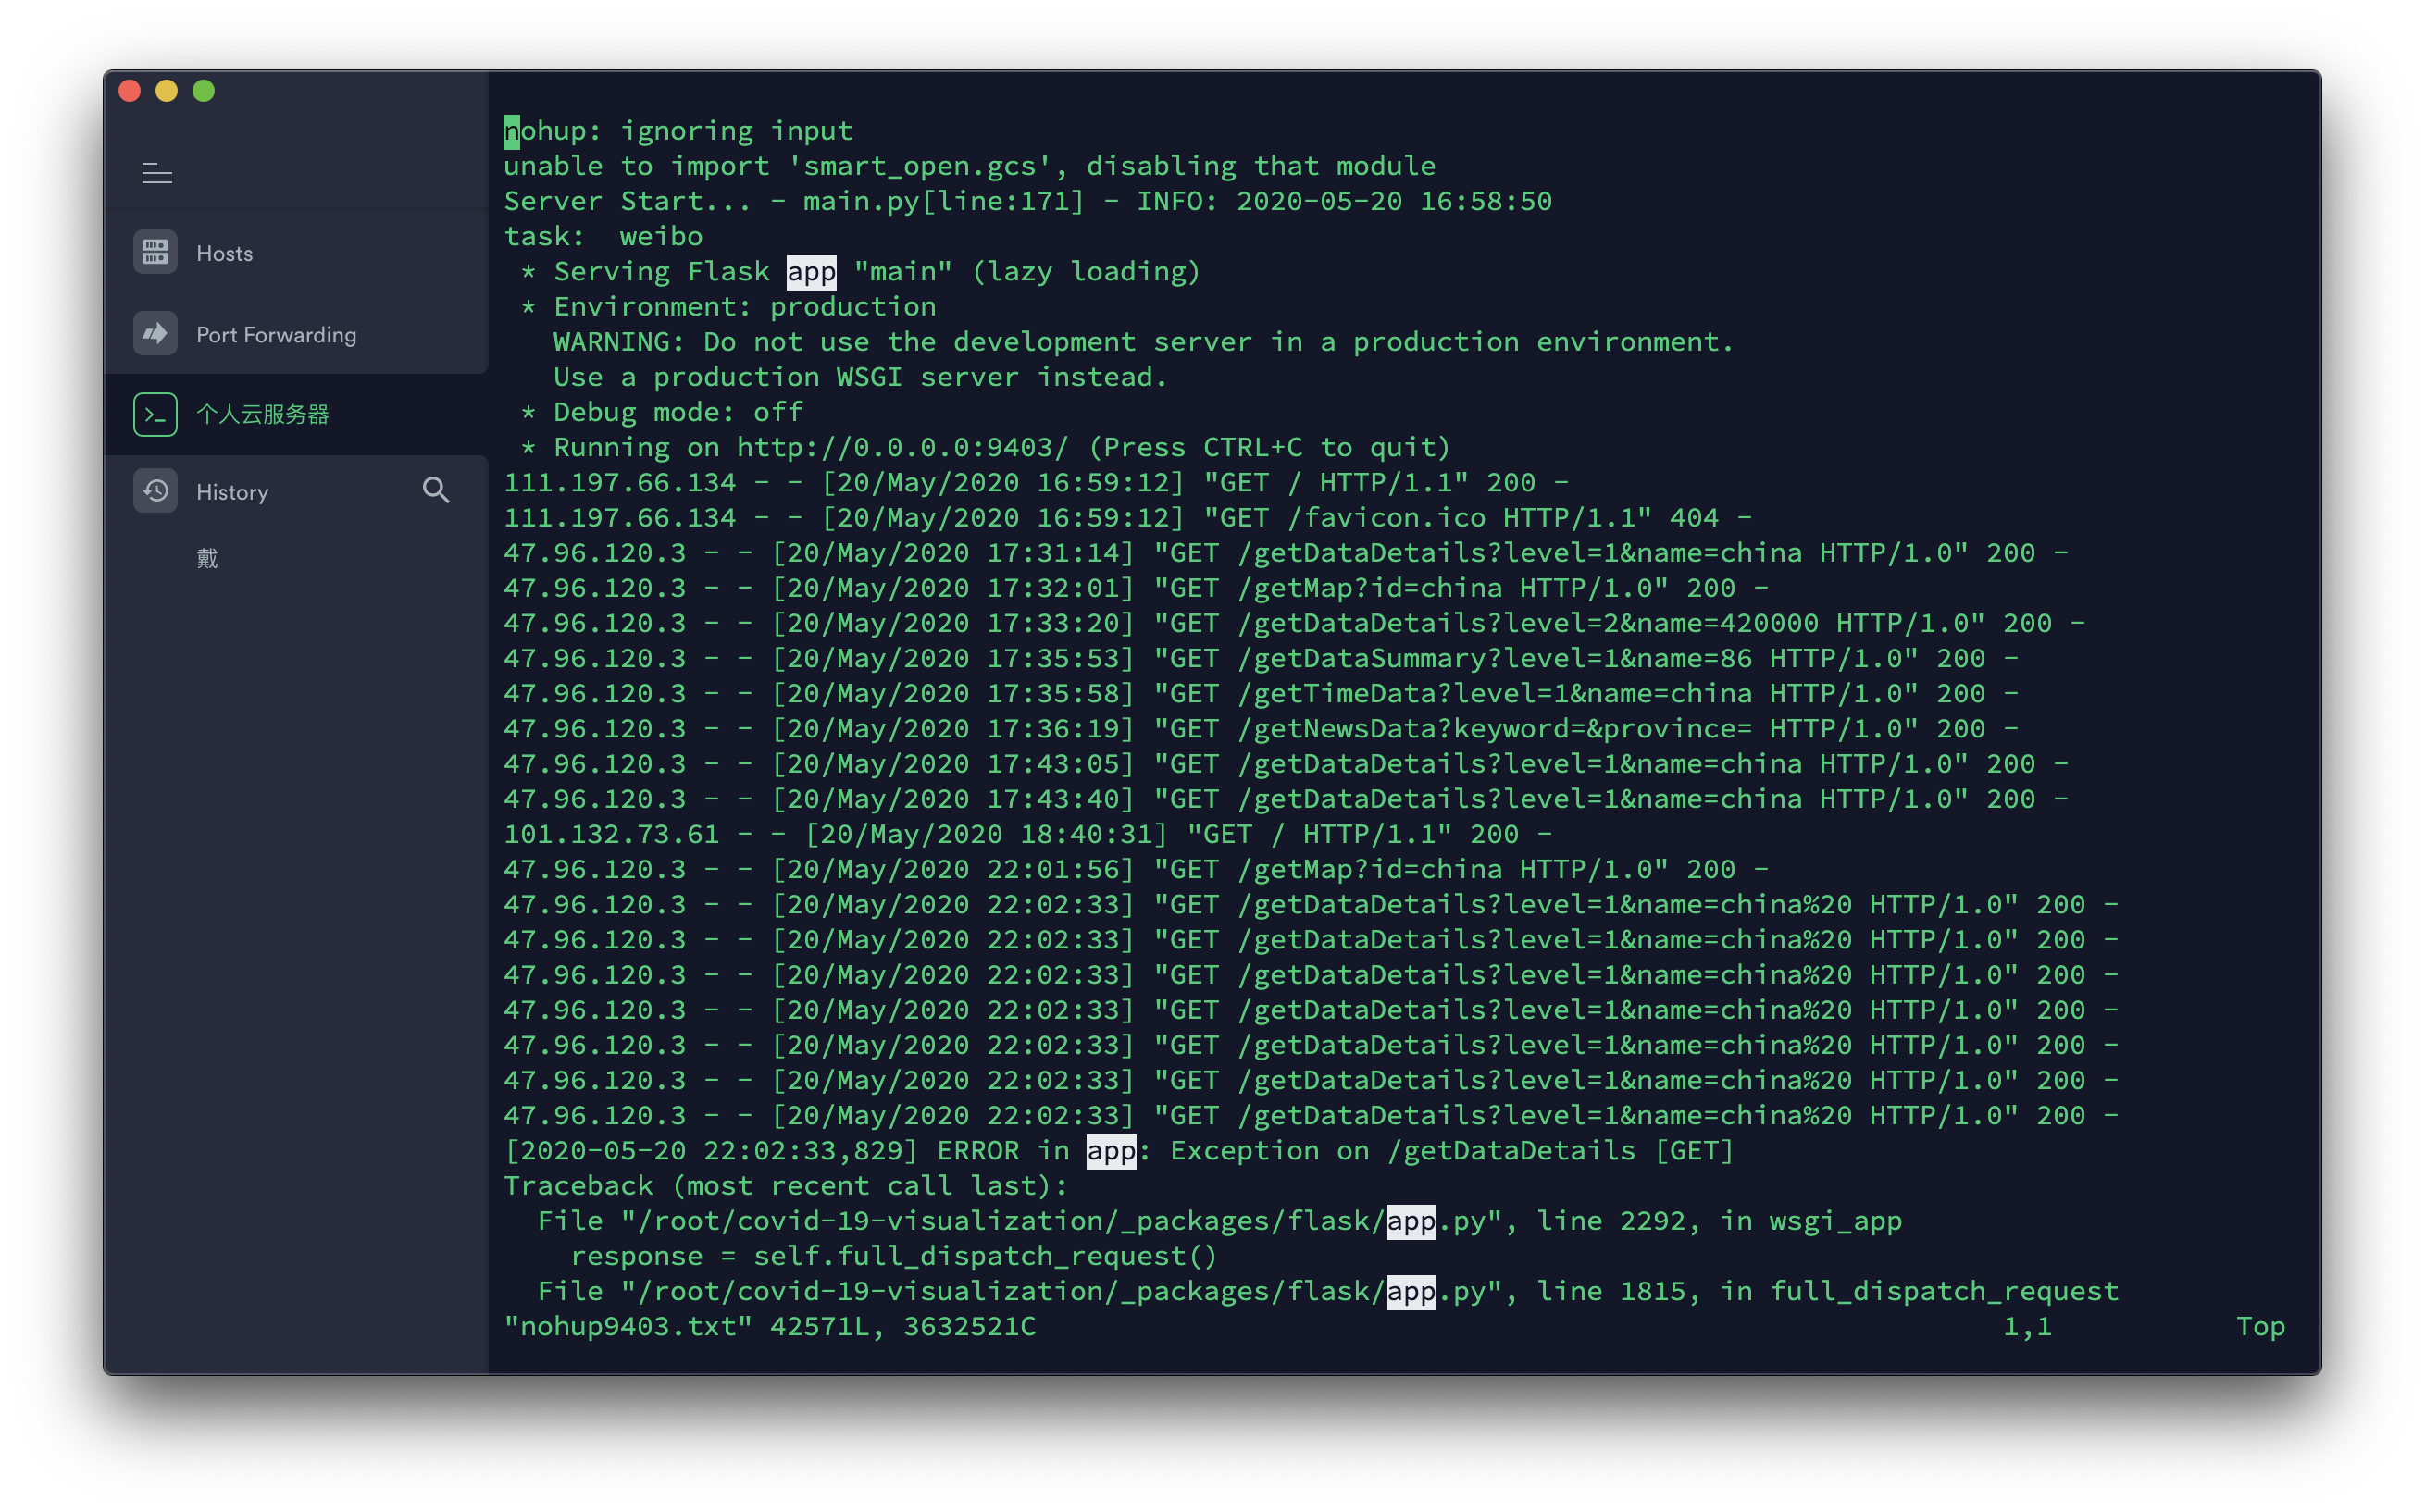
\includegraphics[width=0.6\textwidth]{progress-report-3/log3.png}
\end{figure}

\end{document}